%%%%%%%%%%%%%%%%%%%%%%%%%%%%%%%%%%%%%%%%%%%%%%%%%%%%%%%%%%%%%%%%%%%%%%%%%%%%%%%%
\chapter{Probability and Math Revision}
\label{ap:revision-probability}
%%%%%%%%%%%%%%%%%%%%%%%%%%%%%%%%%%%%%%%%%%%%%%%%%%%%%%%%%%%%%%%%%%%%%%%%%%%%%%%%


%%%%%%%%%%%%%%%%%%%%%%%%%%%%%%%%%%%%%%%%%%%%%%%%%%%%%%%%%%%%%%%%%%%%%%%%%%%%%%%%
\section{Random variable}
We call random variable X a measurable real-valued  function of possible outcomes ($\Omega$ ) defined on a sample space($E$).

\begin{equation}
	X: \Omega \rightarrow E
\end{equation}


%%%%%%%%%%%%%%%%%%%%%%%%%%%%%%%%%%%%%%%%%%%%%%%%%%%%%%%%%%%%%%%%%%%%%%%%%%%%%%%%
\section{Probability Density Function (PDF)}

Let X be a continuous random variable. We say that X is a continuous random variable if there is a function $f (x) $, that satisfies for a set $B = \{b \in \mathbb{R} | b_ {1} \leq b \leq b_ {2}\} $, defined for all $x = \{x \in \mathbb{R}| - \infty \leq x \leq + \infty\} $, having the property: 
\begin{equation}
	P(X \in B) = \int_{b_{1}}^{b_{2}}f(x) dx 
\end{equation}

Where $P$ is the probability function of the random variable $x$. $f(x)$ is called probability density function of the random variable $X$\cite{ross-probability}. 


%%%%%%%%%%%%%%%%%%%%%%%%%%%%%%%%%%%%%%%%%%%%%%%%%%%%%%%%%%%%%%%%%%%%%%%%%%%%%%%%
\section{Cumulative Distribution Function (CDF)}

The Cumulative Distribution Function of a random variable $X$, we represent by $F (x) $ is defined at a given point $\ \in X$ as\cite{ross-probability}: 

\begin{equation}
F(a) = P(X \leq a) = \int_{- \infty}^{a}f(x) dx 
\end{equation}


%%%%%%%%%%%%%%%%%%%%%%%%%%%%%%%%%%%%%%%%%%%%%%%%%%%%%%%%%%%%%%%%%%%%%%%%%%%%%%%%
\section{Expected value, Mean, Variance and Standard Deviation}

Let $X$ be a constinuous random variable, and $f(x)$ be its  density function f (x). Then the expected value of $X$ is defined by:

\begin{equation}
E[X] =  \int_{- \infty}^{+ \infty}xf(x) dx 
\end{equation}

For a random variable normally distributed $X_{normal}$ the result of this definition is equals to the mean $\mu$ of the distribution($E[X_{normal}] = \mu$). For an exponential distribution is equals to the inverse of its rate($E[X_{exponential}] = 1/\lambda$).

The variance of a random variable $X$, denoted by $Var(X)$, is defined by:

\begin{equation}
Var(X) =  E[( X - E[x])^{2}] 
\end{equation}

For a random variable $X$ normally distributed, the variance is equal to its standard deviation ($Var(X) = \sigma^{2}$)\cite{ross-probability}. 

% For a normal distribution the result of this definition is  its mean ($E[X_{normal}] = \mu$), and for an exponential distribution is equals to the inverse of its rate:  ($E[X_{exponential}] = \frac{1}{\lambda}$).

%%%%%%%%%%%%%%%%%%%%%%%%%%%%%%%%%%%%%%%%%%%%%%%%%%%%%%%%%%%%%%%%%%%%%%%%%%%%%%%%
\section{Stochastic Process}

A stochastic process of a random variable represented by $\{X(t)| t \in T\}$ is a collection of random variables. Since $t$ is often interpreted as time, $X (t) $ is usually referred as the state of the process at a given time $t$\cite{ross-probability}.


%%%%%%%%%%%%%%%%%%%%%%%%%%%%%%%%%%%%%%%%%%%%%%%%%%%%%%%%%%%%%%%%%%%%%%%%%%%%%%%%
\section{Self-similarity}

A self similar object has the property of looking "roughly" the same at any scale. Self-similar objects are described by the power law:

\begin{equation}
	N = s^{d}
\end{equation}

where 
\begin{equation}
	d = \frac{\ln{N}}{\ln{s}}
\end{equation}

is the dimension of the scaling law, called  Hausdorff dimension\cite{web-self-similar}. 


\begin{figure*}[ht!]
	\centering
	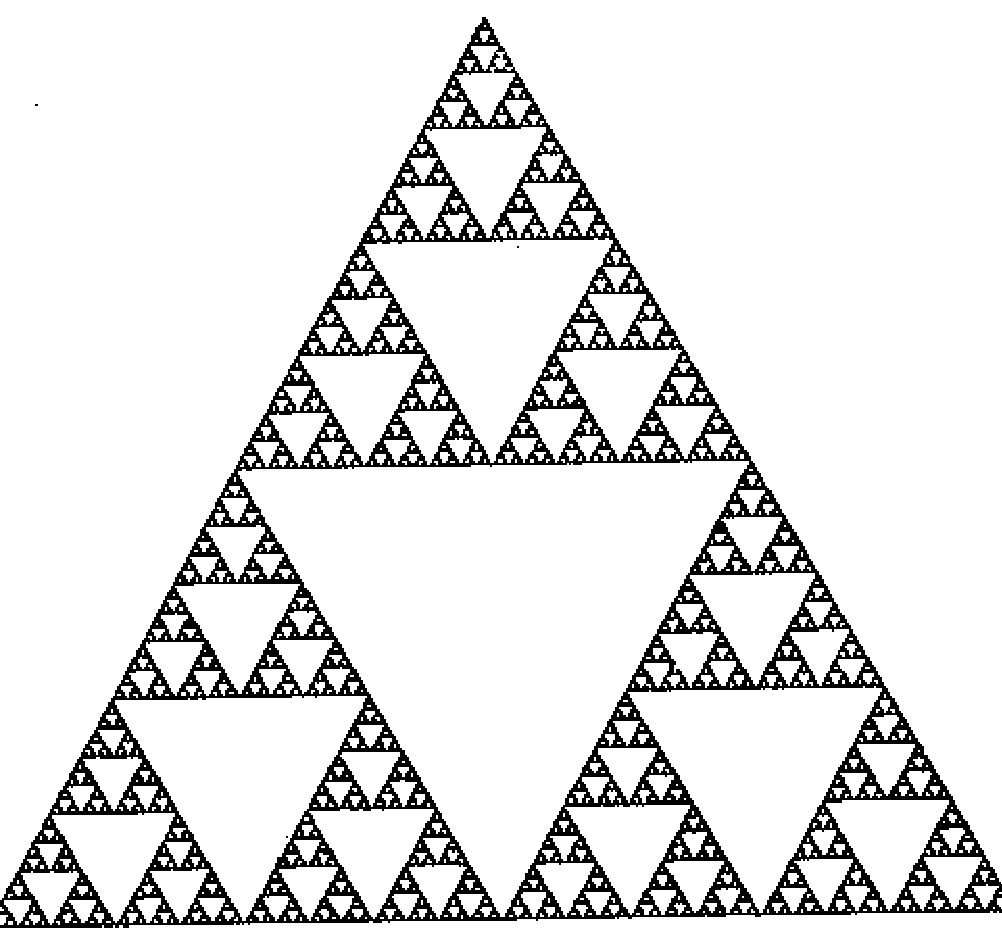
\includegraphics[height=2.0in]{figures/apA/tritrans}
	\caption{This is a classical example of a self-similar figure, caled Sierpinski triangle.}
	\label{fig:self-similar-figure-example}
\end{figure*}


%%%%%%%%%%%%%%%%%%%%%%%%%%%%%%%%%%%%%%%%%%%%%%%%%%%%%%%%%%%%%%%%%%%%%%%%%%%%%%%%
\section{Heavy-tailed distributions}

Heavy tailed distributions are probability distributions whose tails are not exponentially bounded.  A distribution of of a random variable $X$, with cumulative distribution F(x), is said to be heavy tailed, if it satisfies this condition for all $\lambda \in \mathbb{R}$:

\begin{equation}
	\lim_{x\to\infty} e^{\lambda x} (1 - F(x)) = \infty
\end{equation}


%%%%%%%%%%%%%%%%%%%%%%%%%%%%%%%%%%%%%%%%%%%%%%%%%%%%%%%%%%%%%%%%%%%%%%%%%%%%%%%%
\section{\textit{QQplot} analysis}

\textit{QQplot} is used to test if two data-sets comes from a common distribution\cite{web-qqplot}. In our study case, we use to compare empirical data, with theoretical given by model approximations. We show down below the image presented on chapter ~\ref{ch:literature-review} for reference. Looking on how the dot plot behaves compared to the linear line, we can see how well the theoretical plot (the estimated data, on the horizontal axis) represents the actual values (sample data, vertical axis):

\begin{itemize}
\item \textbf{Light-tailed}: the samples still hold a slight heavy-tail effect compared to the estimated by the theoretical values.
\item \textbf{Heavy-tailed}: the samples have a predominant heavy-tail effect compared to the estimated by the theoretical values.
\item \textbf{Linear}: the samples matches the theoretical values.
\item \textbf{Bimodal}: samples present a bimodal pattern.
\item \textbf{Left skew}: small values are underrepresented by the model(~\ref{fig:qqplot-rl-skew}).
\item \textbf{Right skew}: larger values are underrepresented by the model(~\ref{fig:qqplot-rl-skew}).
\end{itemize}

As example, we create a \textit{QQplot} in the figure~\ref{fig:qq-cauchy}, where we use as samples randomly generated data generated by a Cauchy, and as theoretical values, normal random data. Comparing with the figure ~\ref{fig:qqplot-tutorial-ap}, we can identify a heavy tail behavior on the sample data.

\begin{figure*}[ht!]
	\centering
	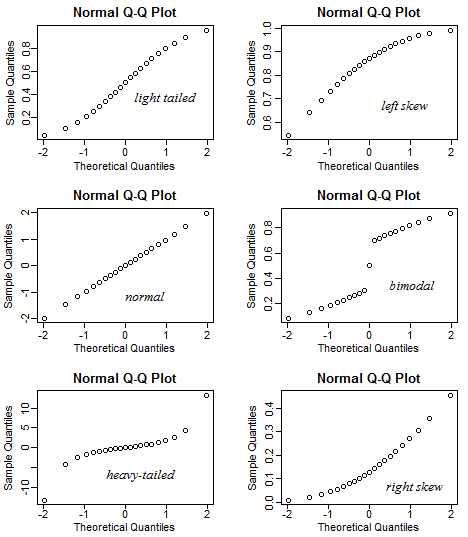
\includegraphics[width=0.55\textwidth]{figures/ch2/qqplot-tutorial}
	\caption{How information about data samples can be extracted from \textit{QQplots}. Depending on the shape of the dot plot,  }
	\label{fig:qqplot-tutorial-ap}
\end{figure*}

\begin{figure*}[ht!]
	\centering
	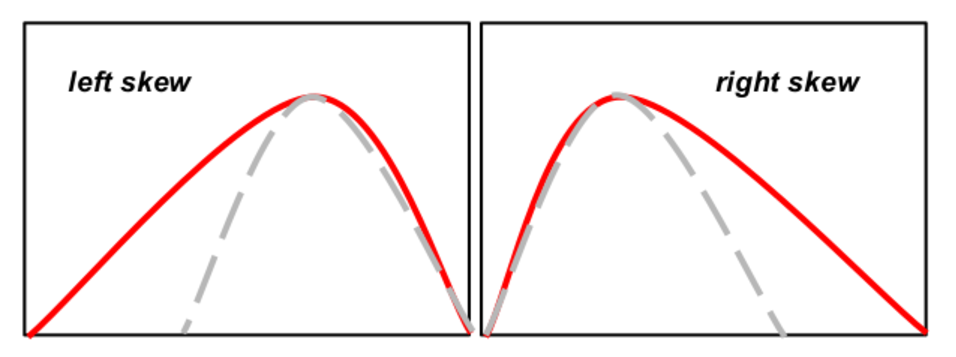
\includegraphics[width=0.5\textwidth]{figures/apA/rl-skew}
	\caption{Shape of a distribution with right and left skew.}
	\label{fig:qqplot-rl-skew}
\end{figure*}

\begin{figure}[t!]
    \centering
    %\subfloat[]{
        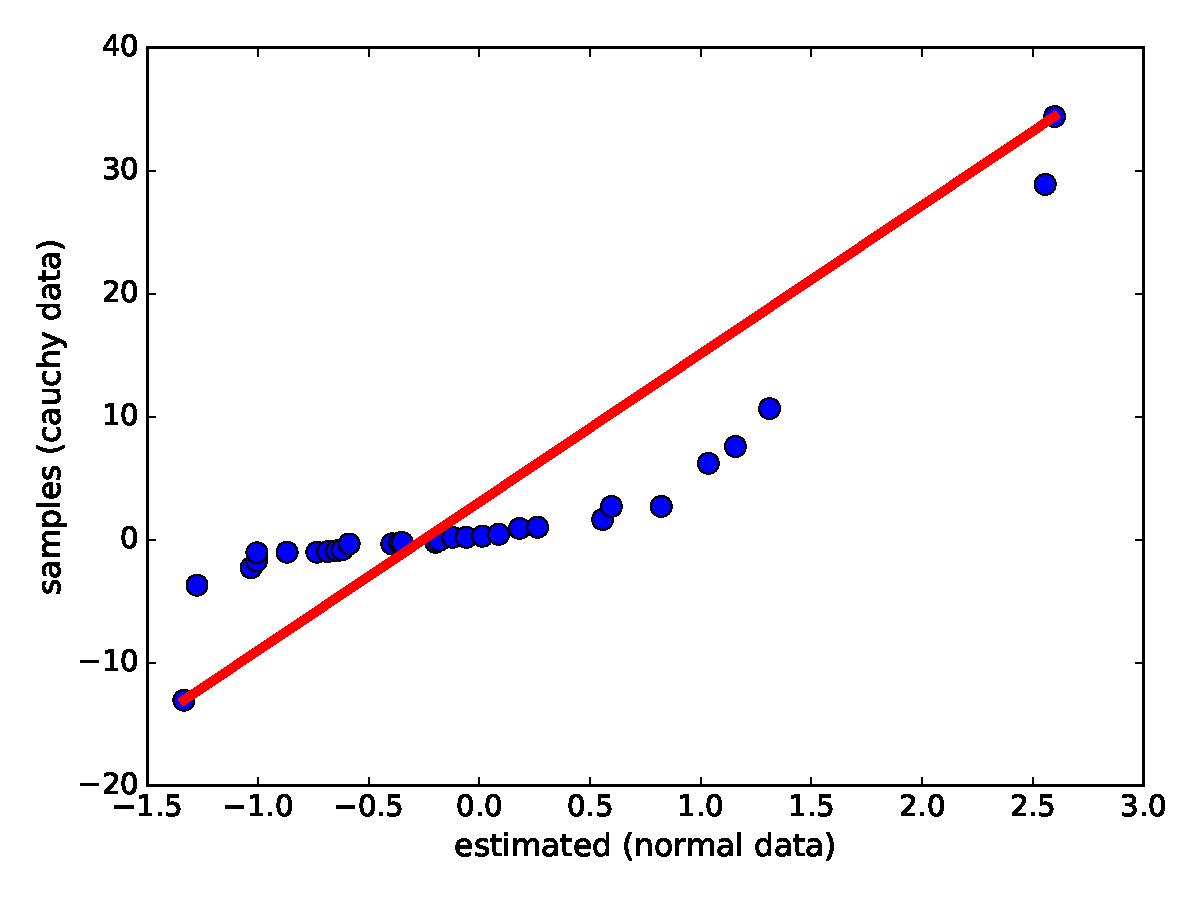
\includegraphics[width=60mm]{figures/apA/qq-c1}
    %    \label{fig:qq-cauchy-1}
    %}
    \hspace{0mm}
    %\subfloat[]{
        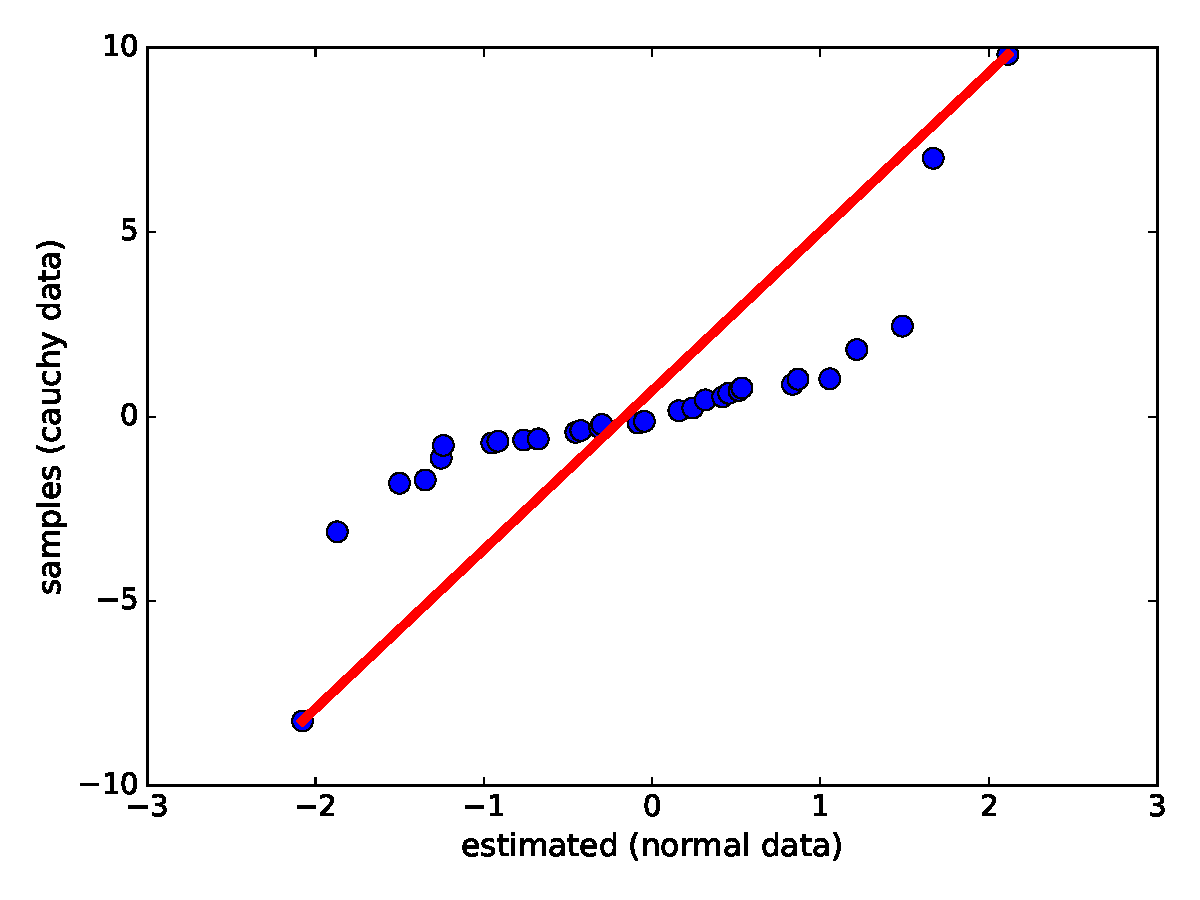
\includegraphics[width=60mm]{figures/apA/qq-c2}
    %    \label{fig:qq-cauchy-2}
    %}
    \caption{QQplot of randomly generated data of a Cauchy process as samples and a normal process as theoretical. We can identify a heavy-tail behavior on the samples, compared to the theoretical.}
    \label{fig:qq-cauchy}
\end{figure}

To generate the plots on figure~\ref{fig:qq-cauchy}, we used Python and the libraries matplotlib and numpy. The code used is shown down below:
\begin{minted}{python}
import numpy as np
import matplotlib.pyplot as plt

nn = sorted(np.random.standard_normal(30))
cc = sorted(np.random.standard_cauchy(30))
nn_max = max(nn)
nn_min = min(nn)
cc_max = max(cc)
cc_min = min(cc)
yy = np.linspace(cc_min, cc_max, num=10)
xx = np.linspace(nn_min, nn_max, num=10)
fig, ax = plt.subplots()
ax.plot(nn, cc, 'bo', markersize=10.0)
ax.plot(xx, yy, 'r-', linewidth=4.0)
plt.xlabel('estimated (normal data)')
plt.ylabel('samples (cauchy data)')
plt.tick_params(labelsize=14)
plt.tight_layout()
plt.show()
\end{minted}



%%%%%%%%%%%%%%%%%%%%%%%%%%%%%%%%%%%%%%%%%%%%%%%%%%%%%%%%%%%%%%%%%%%%%%%%%%%%%%%%
\section{Akaike information criterion (AIC) and Bayesian information criterion (BIC)}

Suppose that we have an statistical model $M$ of some dataset ${\boldsymbol{x} = \{x_1, ..., x_n}\}$, with $n$ independent and identically distributed observations of a random variable $X$. This model can be expressed by a PDF $f(x| \boldsymbol{\theta})$, where $\boldsymbol{\theta}$ a vector of parameter of the PDF, $\boldsymbol{\theta} \in \mathbb{R}^{k}$ ($k$ is the number of parameters). The  likelihood function  of this model $M$ is given by:

\begin{equation}
L(\boldsymbol{\theta}|\boldsymbol{x} ) =  f(x_1|\boldsymbol{\theta})\cdot...\cdot f(x_n|\boldsymbol{\theta}) = \prod_{i = 1}^{n}f(x_i|\boldsymbol{\theta})
\end{equation}

Now, suppose we are trying to estimate the best statistical model, from a set ${M_1, ..., M_n}$, each one whit an estimated vector of parameters  ${\boldsymbol{\hat{\theta_1}}}, ..., {\boldsymbol{\hat{\theta_n}}}$. $AIC$ and $BIC$ are defined by:

\begin{equation}
\label{eq:aic}
AIC = 2k - \ln(L(\boldsymbol{\hat{\theta}}|\boldsymbol{x}))
\end{equation}

\begin{equation}
\label{eq:bic}
BIC = k\ln(n) - \ln(L(\boldsymbol{\hat{\theta}}|\boldsymbol{x}))
\end{equation}

In both cases, the preferred model $M_i$, is the one with the smaller value of $AIC_i$ or $BIC_i$.


%%%%%%%%%%%%%%%%%%%%%%%%%%%%%%%%%%%%%%%%%%%%%%%%%%%%%%%%%%%%%%%%%%%%%%%%%%%%%%%%
\section{Gradient Descendent Algorithm}

Given a linear hypothesis for a dataset:

\begin{equation}
	\boldsymbol{h_{\theta}} = \boldsymbol{\theta}^{T}\boldsymbol{x} 
\end{equation}

were $\boldsymbol{h_{\theta}}, \boldsymbol{\theta}, \boldsymbol{x} \in \mathbb{R}^{m}$. If $m = 2$ we will just have a simple linear equation $h_{\theta}(x) = \theta_{0} + \theta_{1}x$.

The goal of the gradient descendent is to minimize the cost function, defined by:

\begin{equation}
	J(\boldsymbol{\theta}) = \frac{1}{2m} \sum_{i = 1}^{m}  ( \boldsymbol{h_{\theta}}(x^{(i)} - y^{(i)} )^{2}
\end{equation}


To do this, we initialize a $\boldsymbol{\theta_{j}}$ vector (usually with zeros), and repeat this procedure, until $\boldsymbol{\theta_{j}}$ converges:

\begin{equation}
	\boldsymbol{\theta_{j + 1}} := \boldsymbol{\theta_{j}} - \alpha \frac{1}{m} \sum_{i = 1}^{m}  ( \boldsymbol{h_{\theta}}(x^{(i)} - y^{(i)} )x_{j}^{i}
\end{equation}

where $\alpha$ is the step value, typically a small positive number. All values of $\boldsymbol{\theta_{j}}$ must be updated simultaneously. 

